\documentclass[a4paper,12pt]{article}
\usepackage[french]{babel}
\usepackage{amsmath, amssymb}
\usepackage{float} % Ajout du package pour l'option H
\usepackage{xcolor}
\usepackage{graphicx}
\usepackage{tcolorbox}

\setlength{\parindent}{0pt}

\begin{document}

\title{Fiche d'exercice : Masse volumique}
\author{N. Bancel}
\date{Février 2025}

\maketitle

\section{Exercice 1}

\subsection{Problème}


\begin{figure}[H]
    \centering
    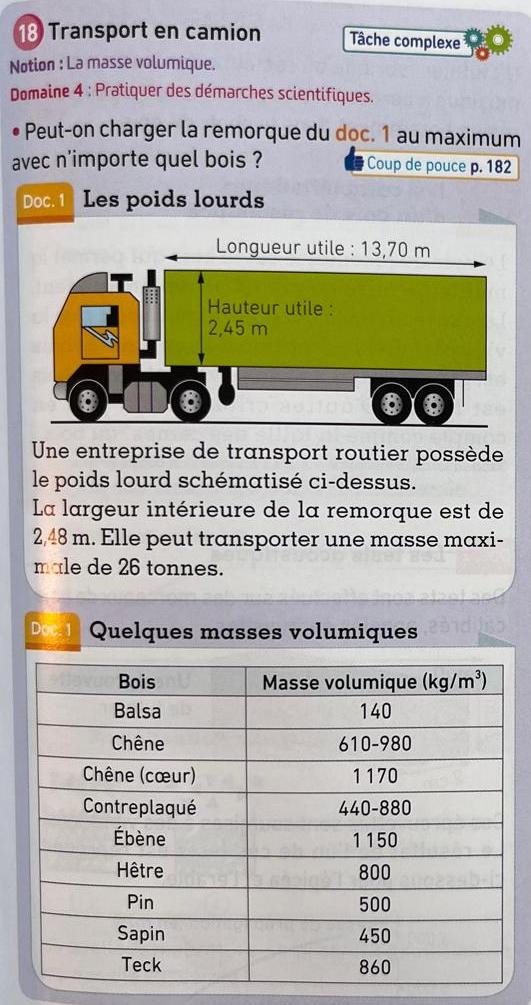
\includegraphics[width=0.4\linewidth]{04_03_02.jpeg}
    \caption{\label{} Énoncé}
  \end{figure}

\subsection{Solution}

\textcolor{blue}{1. Méthode} \\

On veut savoir si la remorque peut être remplie complètement avec n'importe quel type de bois. Pour cela, on va :
\begin{itemize}
    \item Calculer le volume total de la remorque.
    \item Déterminer la masse maximale que la remorque peut supporter.
    \item Comparer avec les masses volumiques des différents bois pour voir lesquels respectent la contrainte de poids.
\end{itemize}

\vspace{0.5cm}

\textcolor{blue}{2. Formules} \\

La formule du volume d'un parallélépipède est :
\[
V = \text{longueur} \times \text{largeur} \times \text{hauteur}
\]

La relation entre la masse, la masse volumique et le volume est :
\[
m = \rho \times V
\]

\vspace{0.5cm}

\textcolor{blue}{3. Application numérique} \\

Calcul du volume de la remorque :
\[
V = 13,70 \times 2,48 \times 2,45
\]
\[
V = 83,1544 \text{ m}^3
\]

La masse maximale supportée par la remorque est de 26 tonnes, soit :
\[
m_{\max} = 26000 \text{ kg}
\]

On en déduit la masse volumique maximale admissible :
\[
\rho_{\max} = \frac{m_{\max}}{V}
\]
\[
\rho_{\max} = \frac{26000}{83,1544} \approx 312,6 \text{ kg/m}^3
\]

\vspace{0.5cm}

\textcolor{blue}{4. Conclusion / Interprétation} \\

On compare cette valeur avec les masses volumiques des bois disponibles :

\begin{itemize}
    \item \textbf{Balsa : 140 kg/m$^3$} \quad Accepté
    \item \textbf{Chêne : 610-980 kg/m$^3$} \quad Trop lourd
    \item \textbf{Chêne (cœur) : 1170 kg/m$^3$} \quad Trop lourd
    \item \textbf{Contreplaqué : 440-880 kg/m$^3$} \quad Trop lourd
    \item \textbf{Ébène : 1150 kg/m$^3$} \quad Trop lourd
    \item \textbf{Hêtre : 800 kg/m$^3$} \quad Trop lourd
    \item \textbf{Pin : 500 kg/m$^3$} \quad Trop lourd
    \item \textbf{Sapin : 450 kg/m$^3$} \quad Trop lourd
    \item \textbf{Teck : 860 kg/m$^3$} \quad Trop lourd
\end{itemize}

\textbf{Conclusion :} Seul le bois de balsa respecte la contrainte de poids et peut être chargé à pleine capacité dans la remorque. Tous les autres bois dépassent la limite autorisée.

\end{document}
